\documentclass[aspectratio=43]{beamer}
%% \documentclass[aspectratio=169]{beamer}
\usetheme[
  block=fill,
  background=light,
  titleformat=smallcaps,
  progressbar=frametitle,
  numbering=none,
]{metropolis}
\setbeamersize{text margin left=.7cm,text margin right=.7cm}
\usepackage{appendixnumberbeamer}

%%%%%%%%%%%%%%%%%%%%%%%%%%%%%%%%%%%%%%%%%%
%% Packages
%%%%%%%%%%%%%%%%%%%%%%%%%%%%%%%%%%%%%%%%%%

\usepackage[backend=bibtex,style=authoryear]{biblatex}

% Tikz
\usepackage{tikz}
\usetikzlibrary{arrows,positioning,matrix,fit,backgrounds,decorations.text,decorations.pathmorphing,calc,shapes}

% Colors
\usepackage{xcolor}
\usepackage{contour}

% Images
\usepackage{graphics}
\graphicspath{{img/}}

% Agda
\usepackage{agda}
\setlength{\mathindent}{0em}
\newfontfamily{\AgdaSerifFont}{Linux Libertine O}
\newfontfamily{\AgdaSansSerifFont}{Linux Biolinum O}
\newfontfamily{\AgdaTypewriterFont}{Linux Biolinum O}
\renewcommand{\AgdaFontStyle}[1]{{\AgdaSansSerifFont{}#1}}
\renewcommand{\AgdaKeywordFontStyle}[1]{{\AgdaSansSerifFont{}#1}}
\renewcommand{\AgdaStringFontStyle}[1]{{\AgdaTypewriterFont{}#1}}
\renewcommand{\AgdaCommentFontStyle}[1]{{\AgdaTypewriterFont{}#1}}
\renewcommand{\AgdaBoundFontStyle}[1]{\textit{\AgdaSerifFont{}#1}}

% Haskell
\usepackage{minted}
\newcommand\hs[1]{\mintinline{haskell}{#1}}
%% \usemintedstyle{friendly}
\usepackage{fontspec}
\setmonofont[Scale=MatchLowercase]{FiraMono-Regular.otf}

% Inference rules
\usepackage{amssymb}
\usepackage{stmaryrd}
\usepackage{proof}
\newenvironment{proposition}[1]
  {\begin{alertblock}{#1}\begin{displaymath}}
  {\end{displaymath}\end{alertblock}}

%%%%%%%%%%%%%%%%%%%%%%%%%%%%%%%%%%%%%%%%%%
%% Macros
%%%%%%%%%%%%%%%%%%%%%%%%%%%%%%%%%%%%%%%%%%
\renewcommand\alert[1]{\textcolor{mLightBrown}{#1}}
\newcommand\todo[1]{\textcolor{red}{#1}}

% My publications
\newcommand\citewtsc{%
\textbf{WTSC @ FC'20}\\
The Extended UTxO Model\\
\scriptsize{\textit{M.Chakravarty, J.Chapman, K.MacKenzie, O.Melkonian, M.P.Jones, P.Wadler}}
}
\newcommand\citeutxoma{%
\textbf{RSC @ ISoLA'20}: \textit{UTxO$_{\textsf{ma}}$: UTxO with Multi-Asset Support}
}
\newcommand\citeeutxoma{%
\textbf{RSC @ ISoLA'20}: \textit{Native Custom Tokens in the Extended UTxO Model}
}
\newcommand\citeagda{%
\textbf{CPP @ POPL'22}\\
\small{Reasonable Agda is Correct Haskell: Intrinsic Program Verification using \textsc{agda2Hs}}\\
\scriptsize{\textit{J.Cockx, O.Melkonian, J.Chapman, U.Norell + TU Delft students}}
}

%%%%%%%%%%%%%%%%%%%%%%%%%%%%%%%%%%%%%%%%%%
%% Fonts
%%%%%%%%%%%%%%%%%%%%%%%%%%%%%%%%%%%%%%%%%%
\usepackage{relsize}
\usepackage[tt=false]{libertine}
\usepackage[libertine]{newtxmath}

\usepackage{yfonts}
\usepackage{xspace}
\newcommand\I{\textgoth{I}\xspace}
\newcommand\II{\textgoth{II}\xspace}
\newcommand\III{\textgoth{III}\xspace}

%----------------------------------------------------------------------------

\title{2$^{nd}$-year PhD Report}
%\subtitle{}
\vspace{-1cm}
\author{Orestis Melkonian}
\date{October 11, 2021}
\titlegraphic{
\vspace*{6cm}

\includegraphics[keepaspectratio=true,height=1.2cm]{uoe}\\
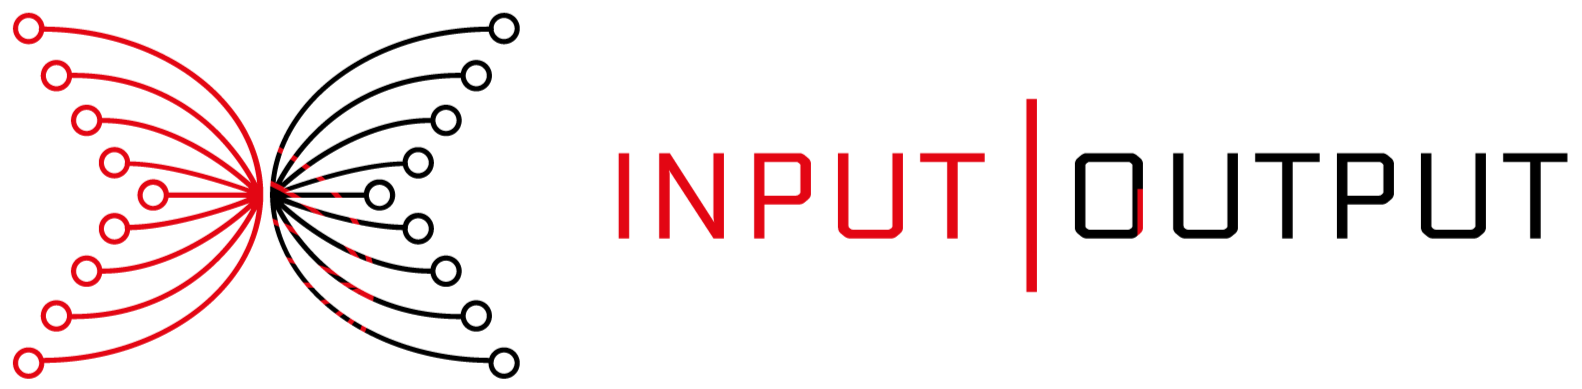
\includegraphics[keepaspectratio=true,height=1.0cm]{iohk}
}

\begin{document}
\begin{center}
\setbeamerfont{title}{size=\large}
\setbeamerfont{subtitle}{size=\small}
\maketitle
\setbeamerfont{title}{size=\Large}
\setbeamerfont{subtitle}{size=\large}
\end{center}

\tikzset{
  % global
  every matrix/.style =
  { ampersand replacement = \&,
    matrix of nodes,
    nodes in empty cells },
  % nodes
  boxx/.style = {align = center},
  box/.style =
  { %draw, rectangle,
    align          = center,
    minimum width  = .5cm,
    minimum height = 1.5cm },
  BG/.style =
  { rectangle,
    inner sep       = 0.2cm,
    rounded corners = 5mm,
    line width      = 1mm },
  MSc/.style =
  { BG, fill=yellow!25, text=yellow!25 },
  MSc-label/.style =
  { label={[name=msc]above left:\contour{yellow!25}{}} },
  PhD/.style =
  { BG, fill=orange!20, text=orange!20 },
  PhD-label/.style =
  { label={[name=phd]below:\contour{orange!20}{}} },
  PhD2/.style =
  { BG, fill=orange!30, text=orange!30 },
  PhD2-label/.style =
  { label={[name=phd]#1:\contour{orange!30}{}} },
  PhD3/.style =
  { BG, fill=green!25, text=green!25 },
  PhD3-label/.style =
  { label={[name=phd]#1:\contour{green!25}{}} },
  greenBox/.style =
  { BG, fill=green!15, },
%%   greenDot/.style =
%%   { BG , left color = red!35, middle color = green!55
%%   , bottom color = green!55, right color = green!55 },
  redDot/.style =
  { BG, draw=red!55, dashed },
  %% font=\small,
  txt/.style    = {align=center},
  note/.style   = {font=\small\itshape},
  accept/.style = {fill = green!15},
  reject/.style = {fill = red!15},
  cit/.style =
  { inner sep = 0.3cm, rounded corners = 2mm, font=\normalsize, align=center },
  % edges
  to/.style = {->, thick},
  squig/.style = {decorate, decoration={zigzag}}
}

\newcommand\bitml{
  \matrix (mat)
    [ column sep = 1.5cm,
      row sep = 2cm,
      every node/.style = txt
    ] {
    \node {\textbf{\underline{Syntax}}};
    \& \node (operA) {};
    \& \node (operB) {};
    \& \node {\textbf{\underline{Game-theoretic}}\\\textbf{\underline{Semantics}}}; \\[-1cm]
    \node (contracts) {BitML\\Contracts};
    \& \node (lts) {Small-step\\LTS};
    \& \node (sm) {Symbolic\\Runs};
    \& \node (ss) {Symbolic\\Strategies}; \\
    \node (transactions) {Bitcoin\\Transactions};
    \& \node (bc) {Blockchain\\Consistency};
    \& \node (cm) {Computational\\Runs};
    \& \node (cs) {Computational\\Strategies}; \\
  };
  \node[fit=(operA)(operB)]{\textbf{\underline{Operational Semantics}}};
  \path
  (contracts) edge[to]
    node[right] (comp) {$\mathcal{C}$}
  (transactions)
  (sm) edge[<->, bend left = 40]
    node[right] (coh) {$\sim$}
  (cm)
  (cm) edge[to]
    node[left] (parsing) {\textit{\alert{parse}}}
  (sm)
  (ss) edge[to]
    node[left] (n) {$\aleph$}
  (cs)
  (coh.east) edge[<->, double]
    node[above] (compsA) {\textit{\alert{computational}}}
    node[below] (compsB) {\textit{\alert{soundness}}}
  (n.west)
  (lts) edge[squig] (sm)
  (bc) edge[squig] (cm)
  ;
}


\section{Year \I: \textit{Recap}}

\begin{frame}{Recap}
Mechanising the meta-theory of two separate objects of study:
  \begin{itemize}
  \item \textbf{BitML}: Bitcoin Modelling Language
  \item The (extended) \textbf{UTxO} model
  \end{itemize}
\end{frame}

\begin{frame}{UTxO [2018-2020]}
\begin{center}
\begin{tikzpicture}
  \utxo
  \begin{pgfonlayer}{background}
    \onslide<+->{
      \node[MSc, MSc-label, fit=(utxo) (eutxo)] {};
      \node[PhD, PhD-label, fit=(iso) (cem)] {};
    }
    \onslide<+>{
      \node[cit, below = of cem] {\citewtsc};
    }
  \end{pgfonlayer}
\end{tikzpicture}
\end{center}
\end{frame}

\begin{frame}{BitML [2018-2020]}
\begin{center}
\begin{tikzpicture}
  \bitml
  \begin{pgfonlayer}{background}
    \onslide<+->{
      \node[MSc, MSc-label, fit=(contracts) (sm)] {};
      \node[PhD, PhD-label, fit=(transactions) (cm)] {};
      \node[PhD, fit=(contracts.south) (comp) (transactions)] {};
    }
  \end{pgfonlayer}
\end{tikzpicture}
\end{center}
\end{frame}

\section{Year \II: \textit{Where I've been...}}

\begin{frame}{UTxO [2020-2021]}
\begin{center}
\begin{tikzpicture}
  \utxo
  \begin{pgfonlayer}{background}
    \onslide<+->{
      \node[MSc, MSc-label, fit=(utxo) (eutxo)] {};
      \node[PhD, PhD-label, fit=(iso) (cem)] {};
    }
  \end{pgfonlayer}
  \begin{pgfonlayer}{background}
    \onslide<+->{
      \node[PhD2, PhD2-label={below}, fit=(l) (cem2)] {};
      %% \node[PhD2, fit=(iso) (cem2)] {};
    }
  \end{pgfonlayer}
  \onslide<+>{
    \node[cit, below = of cem] (utxoma) {\citeutxoma};
    \node[cit, below = 1pt of utxoma] {\citeeutxoma};
  }
\end{tikzpicture}
\end{center}
\end{frame}

\newcommand\froto{$\leftrightarrow$}
\begin{frame}{Separation Logic for UTxO}
\begin{itemize}
\item In collaboration with W.Swierstra (UU) and J.Chapman (IOHK)
\pause
\item[]
\begin{tabular}{ccc}
\textbf{Blockchain} & & \textbf{Concurrency Theory} \\
\hline
ledgers &\froto& computer memory \\
memory locations &\froto& accounts \\
data values &\froto& account balances \\
smart contracts &\froto& programs accessing memory \\
\end{tabular}
\pause
\item[] 
\includegraphics[keepaspectratio=true,height=3ex]{lightbulb}
Transfer results from (Concurrent) Separation Logic!
\end{itemize}
\end{frame}

\begin{frame}{Hoare-style semantics and correspondences}
\begin{center}
\begin{tikzpicture}
  \hoareSemantics
\end{tikzpicture}
\end{center}
\pause
\begin{minipage}{.4\textwidth}
\begin{proposition}{SL: \texttt{[FRAME]} rule}
\infer
  {\{ P * R \} l \{ Q * R \} }
  {%
    l \# R
  & \{ P \} l \{ Q \}
  }
\end{proposition}
\end{minipage}
\pause
\hfill
\begin{minipage}{.4\textwidth}
\begin{proposition}{CSL: \texttt{[PARALLEL]} rule}
\infer
  {\{ P_1 * P_2 \} l \{ Q_1 * Q_2 \} }
  { \deduce{\{ P_1 \} l_1 \{ Q_1 \} }
           {l_1 \parallel l_2 = l}
  & \deduce{\{ P_2 \} l_2 \{ Q_2 \} }
           {l_1 \# P_2 \quad l_2 \# P_1 }
  }
\end{proposition}
\end{minipage}
\end{frame}

\begin{frame}{BitML [2020-2021]}
\begin{center}
\scalebox{.95}{
  \begin{tikzpicture}
  \bitml
  \begin{pgfonlayer}{background}
    \node[MSc, MSc-label, fit=(contracts) (sm)] {};
    \node[PhD, PhD-label, fit=(transactions) (cm)] {};
    \node[PhD, fit=(contracts.south) (comp) (transactions)] {};
    \onslide<2>{
      \node[greenDot, PhD2-label={above right, xshift=-1em}, fit=(cm.north east) (coh) (sm.south east)] {};
    }
  \end{pgfonlayer}
  \end{tikzpicture}
}
\end{center}
\end{frame}

\begin{frame}{BitML: Coherence}
\vspace{-.35cm}
\hspace{-1.4cm}
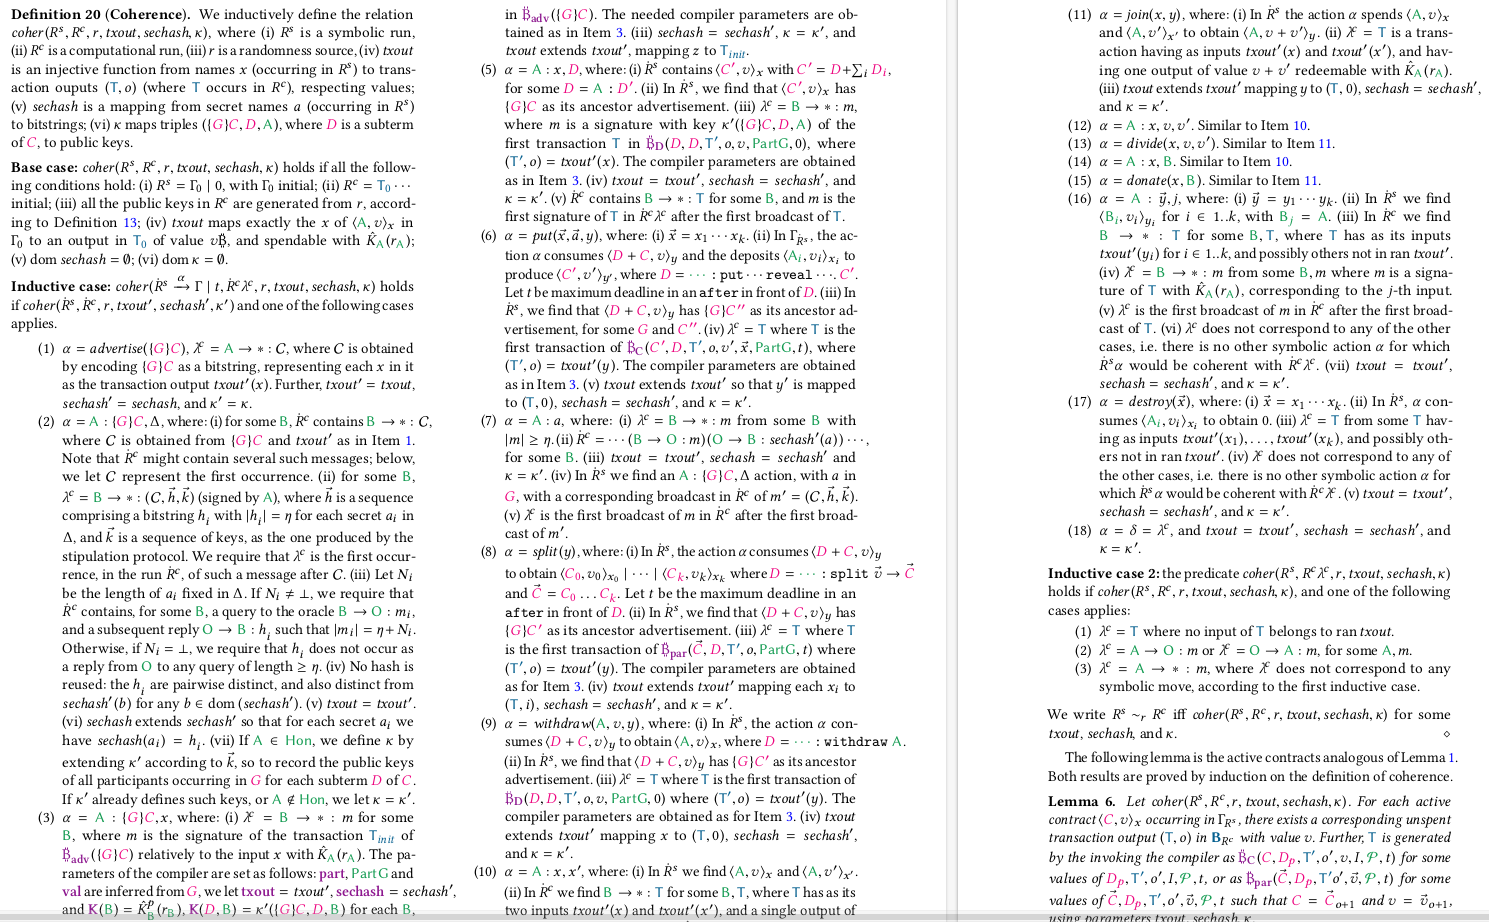
\includegraphics[keepaspectratio=true,width=\paperwidth]{bitml-coherence}
\end{frame}

\begin{code}[hide]%
\>[0]\AgdaKeyword{open}\AgdaSpace{}%
\AgdaKeyword{import}\AgdaSpace{}%
\AgdaModule{Haskell.Prim}\<%
\\
\>[0]\AgdaKeyword{open}\AgdaSpace{}%
\AgdaKeyword{import}\AgdaSpace{}%
\AgdaModule{Haskell.Prim.String}\<%
\\
\>[0]\AgdaKeyword{open}\AgdaSpace{}%
\AgdaKeyword{import}\AgdaSpace{}%
\AgdaModule{Haskell.Prim.Bool}\<%
\\
\>[0]\AgdaKeyword{open}\AgdaSpace{}%
\AgdaKeyword{import}\AgdaSpace{}%
\AgdaModule{Haskell.Prim.List}\<%
\\
\>[0]\AgdaKeyword{open}\AgdaSpace{}%
\AgdaKeyword{import}\AgdaSpace{}%
\AgdaModule{Haskell.Prim.Foldable}\<%
\\
\>[0]\AgdaKeyword{open}\AgdaSpace{}%
\AgdaKeyword{import}\AgdaSpace{}%
\AgdaModule{Haskell.Prim.Maybe}\<%
\\
\>[0]\AgdaKeyword{open}\AgdaSpace{}%
\AgdaKeyword{import}\AgdaSpace{}%
\AgdaModule{Agda.Builtin.Nat}\<%
\\
\>[0]\AgdaKeyword{open}\AgdaSpace{}%
\AgdaKeyword{import}\AgdaSpace{}%
\AgdaModule{Agda.Builtin.Equality}\<%
\\
%
\\[\AgdaEmptyExtraSkip]%
\>[0]\AgdaKeyword{data}\AgdaSpace{}%
\AgdaOperator{\AgdaDatatype{\AgdaUnderscore{}≤\AgdaUnderscore{}}}\AgdaSpace{}%
\AgdaSymbol{:}\AgdaSpace{}%
\AgdaDatatype{Nat}\AgdaSpace{}%
\AgdaSymbol{→}\AgdaSpace{}%
\AgdaDatatype{Nat}\AgdaSpace{}%
\AgdaSymbol{→}\AgdaSpace{}%
\AgdaPrimitive{Set}\AgdaSpace{}%
\AgdaKeyword{where}\<%
\\
\>[0][@{}l@{\AgdaIndent{0}}]%
\>[2]\AgdaInductiveConstructor{zero-≤}\AgdaSpace{}%
\AgdaSymbol{:}\AgdaSpace{}%
\AgdaSymbol{∀}\AgdaSpace{}%
\AgdaSymbol{\{}\AgdaBound{n}\AgdaSymbol{\}}\AgdaSpace{}%
\AgdaSymbol{→}\AgdaSpace{}%
\AgdaInductiveConstructor{zero}\AgdaSpace{}%
\AgdaOperator{\AgdaDatatype{≤}}\AgdaSpace{}%
\AgdaBound{n}\<%
\\
%
\>[2]\AgdaInductiveConstructor{suc-≤}\AgdaSpace{}%
\AgdaSymbol{:}\AgdaSpace{}%
\AgdaSymbol{∀}\AgdaSpace{}%
\AgdaSymbol{\{}\AgdaBound{m}\AgdaSpace{}%
\AgdaBound{n}\AgdaSymbol{\}}\AgdaSpace{}%
\AgdaSymbol{→}\AgdaSpace{}%
\AgdaBound{m}\AgdaSpace{}%
\AgdaOperator{\AgdaDatatype{≤}}\AgdaSpace{}%
\AgdaBound{n}\AgdaSpace{}%
\AgdaSymbol{→}\AgdaSpace{}%
\AgdaInductiveConstructor{suc}\AgdaSpace{}%
\AgdaBound{m}\AgdaSpace{}%
\AgdaOperator{\AgdaDatatype{≤}}\AgdaSpace{}%
\AgdaInductiveConstructor{suc}\AgdaSpace{}%
\AgdaBound{n}\<%
\\
%
\\[\AgdaEmptyExtraSkip]%
\>[0]\AgdaKeyword{data}\AgdaSpace{}%
\AgdaDatatype{Comparison}\AgdaSpace{}%
\AgdaSymbol{\{}\AgdaBound{m}\AgdaSpace{}%
\AgdaBound{n}\AgdaSpace{}%
\AgdaSymbol{:}\AgdaSpace{}%
\AgdaDatatype{Nat}\AgdaSymbol{\}}\AgdaSpace{}%
\AgdaSymbol{:}\AgdaSpace{}%
\AgdaPrimitive{Set}\AgdaSpace{}%
\AgdaKeyword{where}\<%
\\
\>[0][@{}l@{\AgdaIndent{0}}]%
\>[2]\AgdaInductiveConstructor{LT}%
\>[6]\AgdaSymbol{:}\AgdaSpace{}%
\AgdaSymbol{\{}\AgdaBound{pf}\AgdaSpace{}%
\AgdaSymbol{:}\AgdaSpace{}%
\AgdaBound{m}\AgdaSpace{}%
\AgdaOperator{\AgdaDatatype{≤}}\AgdaSpace{}%
\AgdaBound{n}\AgdaSymbol{\}}\AgdaSpace{}%
\AgdaSymbol{→}\AgdaSpace{}%
\AgdaDatatype{Comparison}\AgdaSpace{}%
\AgdaSymbol{\{}\AgdaBound{m}\AgdaSymbol{\}}\AgdaSpace{}%
\AgdaSymbol{\{}\AgdaBound{n}\AgdaSymbol{\}}\<%
\\
%
\>[2]\AgdaInductiveConstructor{EQ}%
\>[6]\AgdaSymbol{:}\AgdaSpace{}%
\AgdaSymbol{\{}\AgdaBound{pf}\AgdaSpace{}%
\AgdaSymbol{:}\AgdaSpace{}%
\AgdaBound{m}\AgdaSpace{}%
\AgdaOperator{\AgdaDatatype{≡}}\AgdaSpace{}%
\AgdaBound{n}\AgdaSymbol{\}}\AgdaSpace{}%
\AgdaSymbol{→}\AgdaSpace{}%
\AgdaDatatype{Comparison}\AgdaSpace{}%
\AgdaSymbol{\{}\AgdaBound{m}\AgdaSymbol{\}}\AgdaSpace{}%
\AgdaSymbol{\{}\AgdaBound{n}\AgdaSymbol{\}}\<%
\\
%
\>[2]\AgdaInductiveConstructor{GT}%
\>[6]\AgdaSymbol{:}\AgdaSpace{}%
\AgdaSymbol{\{}\AgdaBound{pf}\AgdaSpace{}%
\AgdaSymbol{:}\AgdaSpace{}%
\AgdaBound{n}\AgdaSpace{}%
\AgdaOperator{\AgdaDatatype{≤}}\AgdaSpace{}%
\AgdaBound{m}\AgdaSymbol{\}}\AgdaSpace{}%
\AgdaSymbol{→}\AgdaSpace{}%
\AgdaDatatype{Comparison}\AgdaSpace{}%
\AgdaSymbol{\{}\AgdaBound{m}\AgdaSymbol{\}}\AgdaSpace{}%
\AgdaSymbol{\{}\AgdaBound{n}\AgdaSymbol{\}}\<%
\\
\>[0]\AgdaSymbol{\{-\#}\AgdaSpace{}%
\AgdaKeyword{COMPILE}\AgdaSpace{}%
\AgdaKeyword{AGDA2HS}\AgdaSpace{}%
\AgdaDatatype{Comparison}\AgdaSpace{}%
\AgdaSymbol{\#-\}}\<%
\\
%
\\[\AgdaEmptyExtraSkip]%
\>[0]\AgdaFunction{compare}\AgdaSpace{}%
\AgdaSymbol{:}\AgdaSpace{}%
\AgdaSymbol{(}\AgdaBound{m}\AgdaSpace{}%
\AgdaBound{n}\AgdaSpace{}%
\AgdaSymbol{:}\AgdaSpace{}%
\AgdaDatatype{Nat}\AgdaSymbol{)}\AgdaSpace{}%
\AgdaSymbol{→}\AgdaSpace{}%
\AgdaDatatype{Comparison}\AgdaSpace{}%
\AgdaSymbol{\{}\AgdaBound{m}\AgdaSymbol{\}}\AgdaSpace{}%
\AgdaSymbol{\{}\AgdaBound{n}\AgdaSymbol{\}}\<%
\\
\>[0]\AgdaFunction{compare}\AgdaSpace{}%
\AgdaInductiveConstructor{zero}\AgdaSpace{}%
\AgdaInductiveConstructor{zero}\AgdaSpace{}%
\AgdaSymbol{=}\AgdaSpace{}%
\AgdaInductiveConstructor{EQ}\AgdaSpace{}%
\AgdaSymbol{\{}\AgdaArgument{pf}\AgdaSpace{}%
\AgdaSymbol{=}\AgdaSpace{}%
\AgdaInductiveConstructor{refl}\AgdaSymbol{\}}\<%
\\
\>[0]\AgdaFunction{compare}\AgdaSpace{}%
\AgdaInductiveConstructor{zero}\AgdaSpace{}%
\AgdaSymbol{(}\AgdaInductiveConstructor{suc}\AgdaSpace{}%
\AgdaBound{n}\AgdaSymbol{)}\AgdaSpace{}%
\AgdaSymbol{=}\AgdaSpace{}%
\AgdaInductiveConstructor{LT}\AgdaSpace{}%
\AgdaSymbol{\{}\AgdaArgument{pf}\AgdaSpace{}%
\AgdaSymbol{=}\AgdaSpace{}%
\AgdaInductiveConstructor{zero-≤}\AgdaSymbol{\}}\<%
\\
\>[0]\AgdaFunction{compare}\AgdaSpace{}%
\AgdaSymbol{(}\AgdaInductiveConstructor{suc}\AgdaSpace{}%
\AgdaBound{m}\AgdaSymbol{)}\AgdaSpace{}%
\AgdaInductiveConstructor{zero}\AgdaSpace{}%
\AgdaSymbol{=}\AgdaSpace{}%
\AgdaInductiveConstructor{GT}\AgdaSpace{}%
\AgdaSymbol{\{}\AgdaArgument{pf}\AgdaSpace{}%
\AgdaSymbol{=}\AgdaSpace{}%
\AgdaInductiveConstructor{zero-≤}\AgdaSymbol{\}}\<%
\\
\>[0]\AgdaFunction{compare}\AgdaSpace{}%
\AgdaSymbol{(}\AgdaInductiveConstructor{suc}\AgdaSpace{}%
\AgdaBound{m}\AgdaSymbol{)}\AgdaSpace{}%
\AgdaSymbol{(}\AgdaInductiveConstructor{suc}\AgdaSpace{}%
\AgdaBound{n}\AgdaSymbol{)}\AgdaSpace{}%
\AgdaSymbol{=}\AgdaSpace{}%
\AgdaOperator{\AgdaFunction{case}}\AgdaSpace{}%
\AgdaFunction{compare}\AgdaSpace{}%
\AgdaBound{m}\AgdaSpace{}%
\AgdaBound{n}\AgdaSpace{}%
\AgdaOperator{\AgdaFunction{of}}\AgdaSpace{}%
\AgdaSymbol{λ}\AgdaSpace{}%
\AgdaKeyword{where}\<%
\\
\>[0][@{}l@{\AgdaIndent{0}}]%
\>[2]\AgdaSymbol{(}\AgdaInductiveConstructor{LT}\AgdaSpace{}%
\AgdaSymbol{\{}\AgdaArgument{pf}\AgdaSpace{}%
\AgdaSymbol{=}\AgdaSpace{}%
\AgdaBound{m≤n}\AgdaSymbol{\})}%
\>[19]\AgdaSymbol{→}\AgdaSpace{}%
\AgdaInductiveConstructor{LT}\AgdaSpace{}%
\AgdaSymbol{\{}\AgdaArgument{pf}\AgdaSpace{}%
\AgdaSymbol{=}\AgdaSpace{}%
\AgdaInductiveConstructor{suc-≤}\AgdaSpace{}%
\AgdaBound{m≤n}\AgdaSymbol{\}}\<%
\\
%
\>[2]\AgdaSymbol{(}\AgdaInductiveConstructor{EQ}\AgdaSpace{}%
\AgdaSymbol{\{}\AgdaArgument{pf}\AgdaSpace{}%
\AgdaSymbol{=}\AgdaSpace{}%
\AgdaInductiveConstructor{refl}\AgdaSymbol{\})}\AgdaSpace{}%
\AgdaSymbol{→}\AgdaSpace{}%
\AgdaInductiveConstructor{EQ}\AgdaSpace{}%
\AgdaSymbol{\{}\AgdaArgument{pf}\AgdaSpace{}%
\AgdaSymbol{=}\AgdaSpace{}%
\AgdaInductiveConstructor{refl}\AgdaSymbol{\}}\<%
\\
%
\>[2]\AgdaSymbol{(}\AgdaInductiveConstructor{GT}\AgdaSpace{}%
\AgdaSymbol{\{}\AgdaArgument{pf}\AgdaSpace{}%
\AgdaSymbol{=}\AgdaSpace{}%
\AgdaBound{n≤m}\AgdaSymbol{\})}%
\>[19]\AgdaSymbol{→}\AgdaSpace{}%
\AgdaInductiveConstructor{GT}\AgdaSpace{}%
\AgdaSymbol{\{}\AgdaArgument{pf}\AgdaSpace{}%
\AgdaSymbol{=}\AgdaSpace{}%
\AgdaInductiveConstructor{suc-≤}\AgdaSpace{}%
\AgdaBound{n≤m}\AgdaSymbol{\}}\<%
\\
\>[0]\AgdaSymbol{\{-\#}\AgdaSpace{}%
\AgdaKeyword{COMPILE}\AgdaSpace{}%
\AgdaKeyword{AGDA2HS}\AgdaSpace{}%
\AgdaFunction{compare}\AgdaSpace{}%
\AgdaSymbol{\#-\}}\<%
\\
%
\\[\AgdaEmptyExtraSkip]%
\>[0]\AgdaFunction{ShowS}\AgdaSpace{}%
\AgdaSymbol{:}\AgdaSpace{}%
\AgdaPrimitive{Set}\<%
\\
\>[0]\AgdaFunction{ShowS}\AgdaSpace{}%
\AgdaSymbol{=}\AgdaSpace{}%
\AgdaFunction{String}\AgdaSpace{}%
\AgdaSymbol{→}\AgdaSpace{}%
\AgdaFunction{String}\<%
\\
\>[0]\AgdaSymbol{\{-\#}\AgdaSpace{}%
\AgdaKeyword{COMPILE}\AgdaSpace{}%
\AgdaKeyword{AGDA2HS}\AgdaSpace{}%
\AgdaFunction{ShowS}\AgdaSpace{}%
\AgdaSymbol{\#-\}}\<%
\\
%
\\[\AgdaEmptyExtraSkip]%
\>[0]\AgdaFunction{showString}\AgdaSpace{}%
\AgdaSymbol{:}\AgdaSpace{}%
\AgdaFunction{String}\AgdaSpace{}%
\AgdaSymbol{→}\AgdaSpace{}%
\AgdaFunction{ShowS}\<%
\\
\>[0]\AgdaFunction{showString}\AgdaSpace{}%
\AgdaSymbol{=}\AgdaSpace{}%
\AgdaOperator{\AgdaFunction{\AgdaUnderscore{}++\AgdaUnderscore{}}}\<%
\\
\>[0]\AgdaSymbol{\{-\#}\AgdaSpace{}%
\AgdaKeyword{COMPILE}\AgdaSpace{}%
\AgdaKeyword{AGDA2HS}\AgdaSpace{}%
\AgdaFunction{showString}\AgdaSpace{}%
\AgdaSymbol{\#-\}}\<%
\\
%
\\[\AgdaEmptyExtraSkip]%
\>[0]\AgdaFunction{showParen}\AgdaSpace{}%
\AgdaSymbol{:}\AgdaSpace{}%
\AgdaDatatype{Bool}\AgdaSpace{}%
\AgdaSymbol{→}\AgdaSpace{}%
\AgdaFunction{ShowS}\AgdaSpace{}%
\AgdaSymbol{→}\AgdaSpace{}%
\AgdaFunction{ShowS}\<%
\\
\>[0]\AgdaFunction{showParen}\AgdaSpace{}%
\AgdaInductiveConstructor{false}\AgdaSpace{}%
\AgdaBound{s}\AgdaSpace{}%
\AgdaSymbol{=}\AgdaSpace{}%
\AgdaBound{s}\<%
\\
\>[0]\AgdaFunction{showParen}\AgdaSpace{}%
\AgdaInductiveConstructor{true}%
\>[16]\AgdaBound{s}\AgdaSpace{}%
\AgdaSymbol{=}\AgdaSpace{}%
\AgdaFunction{showString}\AgdaSpace{}%
\AgdaString{"("}\AgdaSpace{}%
\AgdaOperator{\AgdaFunction{∘}}\AgdaSpace{}%
\AgdaBound{s}\AgdaSpace{}%
\AgdaOperator{\AgdaFunction{∘}}\AgdaSpace{}%
\AgdaFunction{showString}\AgdaSpace{}%
\AgdaString{")"}\<%
\\
\>[0]\AgdaSymbol{\{-\#}\AgdaSpace{}%
\AgdaKeyword{COMPILE}\AgdaSpace{}%
\AgdaKeyword{AGDA2HS}\AgdaSpace{}%
\AgdaFunction{showParen}\AgdaSpace{}%
\AgdaSymbol{\#-\}}\<%
\\
%
\\[\AgdaEmptyExtraSkip]%
\>[0]\AgdaFunction{defaultShowList}\AgdaSpace{}%
\AgdaSymbol{:}\AgdaSpace{}%
\AgdaSymbol{(}\AgdaGeneralizable{a}\AgdaSpace{}%
\AgdaSymbol{→}\AgdaSpace{}%
\AgdaFunction{ShowS}\AgdaSymbol{)}\AgdaSpace{}%
\AgdaSymbol{→}\AgdaSpace{}%
\AgdaDatatype{List}\AgdaSpace{}%
\AgdaGeneralizable{a}\AgdaSpace{}%
\AgdaSymbol{→}\AgdaSpace{}%
\AgdaFunction{ShowS}\<%
\\
\>[0]\AgdaFunction{defaultShowList}\AgdaSpace{}%
\AgdaSymbol{\AgdaUnderscore{}}%
\>[22]\AgdaInductiveConstructor{[]}%
\>[31]\AgdaSymbol{=}\AgdaSpace{}%
\AgdaFunction{showString}\AgdaSpace{}%
\AgdaString{"[]"}\<%
\\
\>[0]\AgdaFunction{defaultShowList}\AgdaSpace{}%
\AgdaBound{shows}\AgdaSpace{}%
\AgdaSymbol{(}\AgdaBound{x}\AgdaSpace{}%
\AgdaOperator{\AgdaInductiveConstructor{∷}}\AgdaSpace{}%
\AgdaBound{xs}\AgdaSymbol{)}\AgdaSpace{}%
\AgdaSymbol{=}\AgdaSpace{}%
\AgdaFunction{showString}\AgdaSpace{}%
\AgdaString{"["}\AgdaSpace{}%
\AgdaOperator{\AgdaFunction{∘}}\AgdaSpace{}%
\AgdaFunction{foldl}\AgdaSpace{}%
\AgdaSymbol{(λ}\AgdaSpace{}%
\AgdaBound{s}\AgdaSpace{}%
\AgdaBound{x}\AgdaSpace{}%
\AgdaSymbol{→}\AgdaSpace{}%
\AgdaBound{s}\AgdaSpace{}%
\AgdaOperator{\AgdaFunction{∘}}\AgdaSpace{}%
\AgdaFunction{showString}\AgdaSpace{}%
\AgdaString{","}\AgdaSpace{}%
\AgdaOperator{\AgdaFunction{∘}}\AgdaSpace{}%
\AgdaBound{shows}\AgdaSpace{}%
\AgdaBound{x}\AgdaSymbol{)}\AgdaSpace{}%
\AgdaSymbol{(}\AgdaBound{shows}\AgdaSpace{}%
\AgdaBound{x}\AgdaSymbol{)}\AgdaSpace{}%
\AgdaBound{xs}\AgdaSpace{}%
\AgdaOperator{\AgdaFunction{∘}}\AgdaSpace{}%
\AgdaFunction{showString}\AgdaSpace{}%
\AgdaString{"]"}\<%
\\
\>[0]\AgdaSymbol{\{-\#}\AgdaSpace{}%
\AgdaKeyword{COMPILE}\AgdaSpace{}%
\AgdaKeyword{AGDA2HS}\AgdaSpace{}%
\AgdaFunction{defaultShowList}\AgdaSpace{}%
\AgdaSymbol{\#-\}}\<%
\end{code}
\newcommand{\agdaTrees}{%
\begin{code}%
\>[0]\AgdaKeyword{data}\AgdaSpace{}%
\AgdaDatatype{Tree}\AgdaSpace{}%
\AgdaSymbol{\{}\AgdaBound{l}\AgdaSpace{}%
\AgdaBound{u}\AgdaSpace{}%
\AgdaSymbol{:}\AgdaSpace{}%
\AgdaDatatype{Nat}\AgdaSymbol{\}}\AgdaSpace{}%
\AgdaSymbol{:}\AgdaSpace{}%
\AgdaPrimitive{Set}\AgdaSpace{}%
\AgdaKeyword{where}\<%
\\
\>[0][@{}l@{\AgdaIndent{0}}]%
\>[2]\AgdaInductiveConstructor{Leaf}%
\>[8]\AgdaSymbol{:}\AgdaSpace{}%
\AgdaSymbol{\{}\AgdaBound{pf}\AgdaSpace{}%
\AgdaSymbol{:}\AgdaSpace{}%
\AgdaBound{l}\AgdaSpace{}%
\AgdaOperator{\AgdaDatatype{≤}}\AgdaSpace{}%
\AgdaBound{u}\AgdaSymbol{\}}\AgdaSpace{}%
\AgdaSymbol{→}\AgdaSpace{}%
\AgdaDatatype{Tree}\AgdaSpace{}%
\AgdaSymbol{\{}\AgdaBound{l}\AgdaSymbol{\}}\AgdaSpace{}%
\AgdaSymbol{\{}\AgdaBound{u}\AgdaSymbol{\}}\<%
\\
%
\>[2]\AgdaInductiveConstructor{Node}%
\>[8]\AgdaSymbol{:}\AgdaSpace{}%
\AgdaSymbol{(}\AgdaBound{x}\AgdaSpace{}%
\AgdaSymbol{:}\AgdaSpace{}%
\AgdaDatatype{Nat}\AgdaSymbol{)}\<%
\\
\>[2][@{}l@{\AgdaIndent{0}}]%
\>[4]\AgdaSymbol{→}\AgdaSpace{}%
\AgdaDatatype{Tree}\AgdaSpace{}%
\AgdaSymbol{\{}\AgdaBound{l}\AgdaSymbol{\}}\AgdaSpace{}%
\AgdaSymbol{\{}\AgdaBound{x}\AgdaSymbol{\}}\AgdaSpace{}%
\AgdaSymbol{→}\AgdaSpace{}%
\AgdaDatatype{Tree}\AgdaSpace{}%
\AgdaSymbol{\{}\AgdaBound{x}\AgdaSymbol{\}}\AgdaSpace{}%
\AgdaSymbol{\{}\AgdaBound{u}\AgdaSymbol{\}}\<%
\\
%
\>[4]\AgdaSymbol{→}\AgdaSpace{}%
\AgdaDatatype{Tree}\AgdaSpace{}%
\AgdaSymbol{\{}\AgdaBound{l}\AgdaSymbol{\}}\AgdaSpace{}%
\AgdaSymbol{\{}\AgdaBound{u}\AgdaSymbol{\}}\<%
\\
\>[0]\AgdaSymbol{\{-\#}\AgdaSpace{}%
\AgdaKeyword{COMPILE}\AgdaSpace{}%
\AgdaKeyword{AGDA2HS}\AgdaSpace{}%
\AgdaDatatype{Tree}\AgdaSpace{}%
\AgdaSymbol{\#-\}}\<%
\\
%
\\[\AgdaEmptyExtraSkip]%
\>[0]\AgdaFunction{insert}\AgdaSpace{}%
\AgdaSymbol{:}\AgdaSpace{}%
\AgdaSymbol{\{}\AgdaBound{l}\AgdaSpace{}%
\AgdaBound{u}\AgdaSpace{}%
\AgdaSymbol{:}\AgdaSpace{}%
\AgdaDatatype{Nat}\AgdaSymbol{\}}\AgdaSpace{}%
\AgdaSymbol{(}\AgdaBound{x}\AgdaSpace{}%
\AgdaSymbol{:}\AgdaSpace{}%
\AgdaDatatype{Nat}\AgdaSymbol{)}\<%
\\
\>[0][@{}l@{\AgdaIndent{0}}]%
\>[2]\AgdaSymbol{→}\AgdaSpace{}%
\AgdaDatatype{Tree}\AgdaSpace{}%
\AgdaSymbol{\{}\AgdaBound{l}\AgdaSymbol{\}}\AgdaSpace{}%
\AgdaSymbol{\{}\AgdaBound{u}\AgdaSymbol{\}}\<%
\\
%
\>[2]\AgdaSymbol{→}\AgdaSpace{}%
\AgdaSymbol{\{}\AgdaBound{l}\AgdaSpace{}%
\AgdaOperator{\AgdaDatatype{≤}}\AgdaSpace{}%
\AgdaBound{x}\AgdaSymbol{\}}\AgdaSpace{}%
\AgdaSymbol{→}\AgdaSpace{}%
\AgdaSymbol{\{}\AgdaBound{x}\AgdaSpace{}%
\AgdaOperator{\AgdaDatatype{≤}}\AgdaSpace{}%
\AgdaBound{u}\AgdaSymbol{\}}\<%
\\
%
\>[2]\AgdaSymbol{→}\AgdaSpace{}%
\AgdaDatatype{Tree}\AgdaSpace{}%
\AgdaSymbol{\{}\AgdaBound{l}\AgdaSymbol{\}}\AgdaSpace{}%
\AgdaSymbol{\{}\AgdaBound{u}\AgdaSymbol{\}}\<%
\\
\>[0]\AgdaFunction{insert}\AgdaSpace{}%
\AgdaBound{x}\AgdaSpace{}%
\AgdaInductiveConstructor{Leaf}\AgdaSpace{}%
\AgdaSymbol{\{}\AgdaBound{l≤x}\AgdaSymbol{\}}\AgdaSpace{}%
\AgdaSymbol{\{}\AgdaBound{x≤u}\AgdaSymbol{\}}\AgdaSpace{}%
\AgdaSymbol{=}\<%
\\
\>[0][@{}l@{\AgdaIndent{0}}]%
\>[2]\AgdaInductiveConstructor{Node}\AgdaSpace{}%
\AgdaBound{x}\AgdaSpace{}%
\AgdaSymbol{(}\AgdaInductiveConstructor{Leaf}\AgdaSpace{}%
\AgdaSymbol{\{}\AgdaArgument{pf}\AgdaSpace{}%
\AgdaSymbol{=}\AgdaSpace{}%
\AgdaBound{l≤x}\AgdaSymbol{\})}\AgdaSpace{}%
\AgdaSymbol{(}\AgdaInductiveConstructor{Leaf}\AgdaSpace{}%
\AgdaSymbol{\{}\AgdaArgument{pf}\AgdaSpace{}%
\AgdaSymbol{=}\AgdaSpace{}%
\AgdaBound{x≤u}\AgdaSymbol{\})}\<%
\\
\>[0]\AgdaFunction{insert}\AgdaSpace{}%
\AgdaBound{x}\AgdaSpace{}%
\AgdaSymbol{(}\AgdaInductiveConstructor{Node}\AgdaSpace{}%
\AgdaBound{y}\AgdaSpace{}%
\AgdaBound{l}\AgdaSpace{}%
\AgdaBound{r}\AgdaSymbol{)}\AgdaSpace{}%
\AgdaSymbol{\{}\AgdaBound{l≤x}\AgdaSymbol{\}}\AgdaSpace{}%
\AgdaSymbol{\{}\AgdaBound{x≤u}\AgdaSymbol{\}}\AgdaSpace{}%
\AgdaSymbol{=}\<%
\\
\>[0][@{}l@{\AgdaIndent{0}}]%
\>[2]\AgdaOperator{\AgdaFunction{case}}\AgdaSpace{}%
\AgdaFunction{compare}\AgdaSpace{}%
\AgdaBound{x}\AgdaSpace{}%
\AgdaBound{y}\AgdaSpace{}%
\AgdaOperator{\AgdaFunction{of}}\AgdaSpace{}%
\AgdaSymbol{λ}\AgdaSpace{}%
\AgdaKeyword{where}\<%
\\
\>[2][@{}l@{\AgdaIndent{0}}]%
\>[4]\AgdaSymbol{(}\AgdaInductiveConstructor{LT}\AgdaSpace{}%
\AgdaSymbol{\{}\AgdaArgument{pf}\AgdaSpace{}%
\AgdaSymbol{=}\AgdaSpace{}%
\AgdaBound{x≤y}\AgdaSymbol{\})}%
\>[21]\AgdaSymbol{→}\AgdaSpace{}%
\AgdaInductiveConstructor{Node}\AgdaSpace{}%
\AgdaBound{y}\AgdaSpace{}%
\AgdaSymbol{(}\AgdaFunction{insert}\AgdaSpace{}%
\AgdaBound{x}\AgdaSpace{}%
\AgdaBound{l}\AgdaSpace{}%
\AgdaSymbol{\{}\AgdaBound{l≤x}\AgdaSymbol{\}}\AgdaSpace{}%
\AgdaSymbol{\{}\AgdaBound{x≤y}\AgdaSymbol{\})}\AgdaSpace{}%
\AgdaBound{r}\<%
\\
%
\>[4]\AgdaSymbol{(}\AgdaInductiveConstructor{EQ}\AgdaSpace{}%
\AgdaSymbol{\{}\AgdaArgument{pf}\AgdaSpace{}%
\AgdaSymbol{=}\AgdaSpace{}%
\AgdaBound{x≡y}\AgdaSymbol{\})}%
\>[21]\AgdaSymbol{→}\AgdaSpace{}%
\AgdaInductiveConstructor{Node}\AgdaSpace{}%
\AgdaBound{y}\AgdaSpace{}%
\AgdaBound{l}\AgdaSpace{}%
\AgdaBound{r}\<%
\\
%
\>[4]\AgdaSymbol{(}\AgdaInductiveConstructor{GT}\AgdaSpace{}%
\AgdaSymbol{\{}\AgdaArgument{pf}\AgdaSpace{}%
\AgdaSymbol{=}\AgdaSpace{}%
\AgdaBound{y≤x}\AgdaSymbol{\})}%
\>[21]\AgdaSymbol{→}\AgdaSpace{}%
\AgdaInductiveConstructor{Node}\AgdaSpace{}%
\AgdaBound{y}\AgdaSpace{}%
\AgdaBound{l}\AgdaSpace{}%
\AgdaSymbol{(}\AgdaFunction{insert}\AgdaSpace{}%
\AgdaBound{x}\AgdaSpace{}%
\AgdaBound{r}\AgdaSpace{}%
\AgdaSymbol{\{}\AgdaBound{y≤x}\AgdaSymbol{\}}\AgdaSpace{}%
\AgdaSymbol{\{}\AgdaBound{x≤u}\AgdaSymbol{\})}\<%
\\
\>[0]\AgdaSymbol{\{-\#}\AgdaSpace{}%
\AgdaKeyword{COMPILE}\AgdaSpace{}%
\AgdaKeyword{AGDA2HS}\AgdaSpace{}%
\AgdaFunction{insert}\AgdaSpace{}%
\AgdaSymbol{\#-\}}\<%
\end{code}}
\newcommand{\agdaClasses}{%
\begin{code}%
\>[0]\AgdaKeyword{record}\AgdaSpace{}%
\AgdaRecord{Show}\AgdaSpace{}%
\AgdaSymbol{(}\AgdaBound{a}\AgdaSpace{}%
\AgdaSymbol{:}\AgdaSpace{}%
\AgdaPrimitive{Set}\AgdaSymbol{)}\AgdaSpace{}%
\AgdaSymbol{:}\AgdaSpace{}%
\AgdaPrimitive{Set}\AgdaSpace{}%
\AgdaKeyword{where}\<%
\\
\>[0][@{}l@{\AgdaIndent{0}}]%
\>[2]\AgdaKeyword{field}%
\>[9]\AgdaField{show}%
\>[20]\AgdaSymbol{:}\AgdaSpace{}%
\AgdaBound{a}\AgdaSpace{}%
\AgdaSymbol{→}\AgdaSpace{}%
\AgdaFunction{String}\<%
\\
%
\>[9]\AgdaField{showsPrec}%
\>[20]\AgdaSymbol{:}\AgdaSpace{}%
\AgdaDatatype{Nat}\AgdaSpace{}%
\AgdaSymbol{→}\AgdaSpace{}%
\AgdaBound{a}\AgdaSpace{}%
\AgdaSymbol{→}\AgdaSpace{}%
\AgdaFunction{ShowS}\<%
\\
%
\>[9]\AgdaField{showList}%
\>[20]\AgdaSymbol{:}\AgdaSpace{}%
\AgdaDatatype{List}\AgdaSpace{}%
\AgdaBound{a}\AgdaSpace{}%
\AgdaSymbol{→}\AgdaSpace{}%
\AgdaFunction{ShowS}\<%
\\
%
\\[\AgdaEmptyExtraSkip]%
\>[0]\AgdaKeyword{record}\AgdaSpace{}%
\AgdaRecord{Show₁}\AgdaSpace{}%
\AgdaSymbol{(}\AgdaBound{a}\AgdaSpace{}%
\AgdaSymbol{:}\AgdaSpace{}%
\AgdaPrimitive{Set}\AgdaSymbol{)}\AgdaSpace{}%
\AgdaSymbol{:}\AgdaSpace{}%
\AgdaPrimitive{Set}\AgdaSpace{}%
\AgdaKeyword{where}\<%
\\
\>[0][@{}l@{\AgdaIndent{0}}]%
\>[2]\AgdaKeyword{field}\AgdaSpace{}%
\AgdaField{showsPrec}\AgdaSpace{}%
\AgdaSymbol{:}\AgdaSpace{}%
\AgdaDatatype{Nat}\AgdaSpace{}%
\AgdaSymbol{→}\AgdaSpace{}%
\AgdaBound{a}\AgdaSpace{}%
\AgdaSymbol{→}\AgdaSpace{}%
\AgdaFunction{ShowS}\<%
\\
%
\\[\AgdaEmptyExtraSkip]%
%
\>[2]\AgdaFunction{show}\AgdaSpace{}%
\AgdaSymbol{:}\AgdaSpace{}%
\AgdaBound{a}\AgdaSpace{}%
\AgdaSymbol{→}\AgdaSpace{}%
\AgdaFunction{String}\<%
\\
%
\>[2]\AgdaFunction{show}\AgdaSpace{}%
\AgdaBound{x}\AgdaSpace{}%
\AgdaSymbol{=}\AgdaSpace{}%
\AgdaField{showsPrec}\AgdaSpace{}%
\AgdaNumber{0}\AgdaSpace{}%
\AgdaBound{x}\AgdaSpace{}%
\AgdaString{""}\<%
\\
%
\\[\AgdaEmptyExtraSkip]%
%
\>[2]\AgdaFunction{showList}\AgdaSpace{}%
\AgdaSymbol{:}\AgdaSpace{}%
\AgdaDatatype{List}\AgdaSpace{}%
\AgdaBound{a}\AgdaSpace{}%
\AgdaSymbol{→}\AgdaSpace{}%
\AgdaFunction{ShowS}\<%
\\
%
\>[2]\AgdaFunction{showList}\AgdaSpace{}%
\AgdaSymbol{=}\AgdaSpace{}%
\AgdaFunction{defaultShowList}\AgdaSpace{}%
\AgdaSymbol{(}\AgdaField{showsPrec}\AgdaSpace{}%
\AgdaNumber{0}\AgdaSymbol{)}\<%
\\
%
\\[\AgdaEmptyExtraSkip]%
\>[0]\AgdaKeyword{record}\AgdaSpace{}%
\AgdaRecord{Show₂}\AgdaSpace{}%
\AgdaSymbol{(}\AgdaBound{a}\AgdaSpace{}%
\AgdaSymbol{:}\AgdaSpace{}%
\AgdaPrimitive{Set}\AgdaSymbol{)}\AgdaSpace{}%
\AgdaSymbol{:}\AgdaSpace{}%
\AgdaPrimitive{Set}\AgdaSpace{}%
\AgdaKeyword{where}\<%
\\
\>[0][@{}l@{\AgdaIndent{0}}]%
\>[2]\AgdaKeyword{field}\AgdaSpace{}%
\AgdaField{show}\AgdaSpace{}%
\AgdaSymbol{:}\AgdaSpace{}%
\AgdaBound{a}\AgdaSpace{}%
\AgdaSymbol{→}\AgdaSpace{}%
\AgdaFunction{String}\<%
\\
%
\\[\AgdaEmptyExtraSkip]%
%
\>[2]\AgdaFunction{showsPrec}\AgdaSpace{}%
\AgdaSymbol{:}\AgdaSpace{}%
\AgdaDatatype{Nat}\AgdaSpace{}%
\AgdaSymbol{→}\AgdaSpace{}%
\AgdaBound{a}\AgdaSpace{}%
\AgdaSymbol{→}\AgdaSpace{}%
\AgdaFunction{ShowS}\<%
\\
%
\>[2]\AgdaFunction{showsPrec}\AgdaSpace{}%
\AgdaSymbol{\AgdaUnderscore{}}\AgdaSpace{}%
\AgdaBound{x}\AgdaSpace{}%
\AgdaBound{s}\AgdaSpace{}%
\AgdaSymbol{=}\AgdaSpace{}%
\AgdaField{show}\AgdaSpace{}%
\AgdaBound{x}\AgdaSpace{}%
\AgdaOperator{\AgdaFunction{++}}\AgdaSpace{}%
\AgdaBound{s}\<%
\\
%
\\[\AgdaEmptyExtraSkip]%
%
\>[2]\AgdaFunction{showList}\AgdaSpace{}%
\AgdaSymbol{:}\AgdaSpace{}%
\AgdaDatatype{List}\AgdaSpace{}%
\AgdaBound{a}\AgdaSpace{}%
\AgdaSymbol{→}\AgdaSpace{}%
\AgdaFunction{ShowS}\<%
\\
%
\>[2]\AgdaFunction{showList}\AgdaSpace{}%
\AgdaSymbol{=}\AgdaSpace{}%
\AgdaFunction{defaultShowList}\AgdaSpace{}%
\AgdaSymbol{(}\AgdaFunction{showsPrec}\AgdaSpace{}%
\AgdaNumber{0}\AgdaSymbol{)}\<%
\\
%
\\[\AgdaEmptyExtraSkip]%
\>[0]\AgdaKeyword{open}\AgdaSpace{}%
\AgdaModule{Show}\AgdaSpace{}%
\AgdaSymbol{\{\{...\}\}}\<%
\\
\>[0]\AgdaSymbol{\{-\#}\AgdaSpace{}%
\AgdaKeyword{COMPILE}\AgdaSpace{}%
\AgdaKeyword{AGDA2HS}\AgdaSpace{}%
\AgdaRecord{Show}\AgdaSpace{}%
\AgdaPragma{class}\AgdaSpace{}%
\AgdaPragma{Show₁}\AgdaSpace{}%
\AgdaPragma{Show₂}\AgdaSpace{}%
\AgdaSymbol{\#-\}}\<%
\\
%
\\[\AgdaEmptyExtraSkip]%
\>[0]\AgdaKeyword{instance}\<%
\\
\>[0][@{}l@{\AgdaIndent{0}}]%
\>[2]\AgdaFunction{ShowMaybe}\AgdaSpace{}%
\AgdaSymbol{:}\AgdaSpace{}%
\AgdaSymbol{\{\{}\AgdaRecord{Show}\AgdaSpace{}%
\AgdaGeneralizable{a}\AgdaSymbol{\}\}}\AgdaSpace{}%
\AgdaSymbol{→}\AgdaSpace{}%
\AgdaRecord{Show}\AgdaSpace{}%
\AgdaSymbol{(}\AgdaDatatype{Maybe}\AgdaSpace{}%
\AgdaGeneralizable{a}\AgdaSymbol{)}\<%
\\
%
\>[2]\AgdaFunction{ShowMaybe}\AgdaSpace{}%
\AgdaSymbol{\{}\AgdaArgument{a}\AgdaSpace{}%
\AgdaSymbol{=}\AgdaSpace{}%
\AgdaBound{a}\AgdaSymbol{\}}\AgdaSpace{}%
\AgdaSymbol{=}\AgdaSpace{}%
\AgdaKeyword{record}\AgdaSpace{}%
\AgdaSymbol{\{}\AgdaModule{Show₁}\AgdaSpace{}%
\AgdaFunction{s₁}\AgdaSymbol{\}}\<%
\\
\>[2][@{}l@{\AgdaIndent{0}}]%
\>[4]\AgdaKeyword{where}\<%
\\
%
\>[4]\AgdaFunction{s₁}\AgdaSpace{}%
\AgdaSymbol{:}\AgdaSpace{}%
\AgdaRecord{Show₁}\AgdaSpace{}%
\AgdaSymbol{(}\AgdaDatatype{Maybe}\AgdaSpace{}%
\AgdaBound{a}\AgdaSymbol{)}\<%
\\
%
\>[4]\AgdaFunction{s₁}\AgdaSpace{}%
\AgdaSymbol{.}\AgdaField{Show₁.showsPrec}\AgdaSpace{}%
\AgdaBound{n}\AgdaSpace{}%
\AgdaSymbol{=}\AgdaSpace{}%
\AgdaSymbol{λ}\AgdaSpace{}%
\AgdaKeyword{where}\<%
\\
\>[4][@{}l@{\AgdaIndent{0}}]%
\>[6]\AgdaInductiveConstructor{Nothing}%
\>[16]\AgdaSymbol{→}\AgdaSpace{}%
\AgdaFunction{showString}\AgdaSpace{}%
\AgdaString{"nothing"}\<%
\\
%
\>[6]\AgdaSymbol{(}\AgdaInductiveConstructor{Just}\AgdaSpace{}%
\AgdaBound{x}\AgdaSymbol{)}%
\>[16]\AgdaSymbol{→}\AgdaSpace{}%
\AgdaFunction{showParen}\AgdaSpace{}%
\AgdaInductiveConstructor{true}\<%
\\
\>[6][@{}l@{\AgdaIndent{0}}]%
\>[8]\AgdaSymbol{(}\AgdaFunction{showString}\AgdaSpace{}%
\AgdaString{"just\ "}\AgdaSpace{}%
\AgdaOperator{\AgdaFunction{∘}}\AgdaSpace{}%
\AgdaPostulate{showsPrec}\AgdaSpace{}%
\AgdaNumber{10}\AgdaSpace{}%
\AgdaBound{x}\AgdaSymbol{)}\<%
\\
\>[0]\AgdaSymbol{\{-\#}\AgdaSpace{}%
\AgdaKeyword{COMPILE}\AgdaSpace{}%
\AgdaKeyword{AGDA2HS}\AgdaSpace{}%
\AgdaFunction{ShowMaybe}\AgdaSpace{}%
\AgdaSymbol{\#-\}}\<%
\end{code}}

\setlength{\AgdaEmptySkip}{1em}
\renewcommand{\AgdaCodeStyle}{\scriptsize}
\setminted[haskell]{fontsize=\tiny}
\begin{frame}[fragile]{agda2hs}
\begin{minipage}[l]{.5\textwidth}
\agdaTrees{}
\end{minipage}
\hfill\vline\hfill
\begin{minipage}[r]{.4\textwidth}
\begin{minted}{haskell}
data Tree = Leaf
          | Node Natural Tree Tree

insert :: Natural -> Tree -> Tree
insert x Leaf = Node x Leaf Leaf
insert x (Node y l r)
  = case compare x y of
      LT -> Node y (insert x l) r
      EQ -> Node x l r
      GT -> Node y l (insert x r)
\end{minted}
\end{minipage}
\end{frame}

\setlength{\AgdaEmptySkip}{0em}
\renewcommand{\AgdaCodeStyle}{\tiny}
\setminted[haskell]{fontsize=\tiny}
\begin{frame}[fragile]{agda2hs: typeclasses}
\begin{minipage}[l]{.4\textwidth}
\agdaClasses{}
\end{minipage}
\hfill\vline\hfill
\begin{minipage}[r]{.5\textwidth}
\begin{minted}{haskell}
class Show a where
  show :: a -> String
  showsPrec :: Natural -> a -> ShowS
  showList :: [a] -> ShowS
  {-# MINIMAL showsPrec | show #-}
  show x = showsPrec 0 x ""
  showList = defaultShowList (showsPrec 0)
  showsPrec _ x s = show x ++ s

instance (Show a) => Show (Maybe a) where
  showsPrec n = \case
    Nothing -> showString "nothing"
    (Just x) -> showParen True
      (showString "just " . showsPrec 10 x)
\end{minted}
\end{minipage}
\pause
\begin{center}
\begin{tikzpicture}[overlay, remember picture]
  %% \tikzset{shift={(page.center)},yshift=-1.5cm}
  \begin{pgfonlayer}{background}
    %% \node[cit,xshift=.3\textwidth,yshift=.3\textheight] {\citeagda};
    \node[cit] at (current page.center) {\citeagda};
  \end{pgfonlayer}
\end{tikzpicture}
\end{center}
\end{frame}

\setminted[yaml]{fontsize=\footnotesize}
\begin{frame}[fragile]{\texttt{setup-agda:} CI infrastructure for Agda}
\begin{minted}{yaml}
name: CI
on: push: {branches: master}
jobs:
  build-deploy:
    runs-on: ubuntu-latest
    steps:
      - uses: actions/checkout@v2.3.1
      - uses: omelkonian/setup-agda@v0.1
        with:
          agda-version: 2.6.1.3
          stdlib-version: 1.6
          libraries: |
            omelkonian/formal-prelude#92ef
            omelkonian/formal-bitcoin#0341
            omelkonian/formal-bitml#4382
          main: Main
          token: ${{ secrets.GITHUB_TOKEN }}
\end{minted}
\end{frame}

\newcommand\agdaSolve{%
\begin{code}%
\>[0]\AgdaKeyword{open}\AgdaSpace{}%
\AgdaKeyword{import}\AgdaSpace{}%
\AgdaModule{Prelude.Init}\AgdaSpace{}%
\AgdaKeyword{using}\AgdaSpace{}%
\AgdaSymbol{(}\AgdaDatatype{List}\AgdaSymbol{)}\<%
\\
\>[0]\AgdaKeyword{open}\AgdaSpace{}%
\AgdaKeyword{import}\AgdaSpace{}%
\AgdaModule{Prelude.Semigroup}\<%
\\
\>[0]\AgdaKeyword{open}\AgdaSpace{}%
\AgdaKeyword{import}\AgdaSpace{}%
\AgdaModule{Prelude.Membership}\<%
\\
\>[0]\AgdaKeyword{open}\AgdaSpace{}%
\AgdaKeyword{import}\AgdaSpace{}%
\AgdaModule{Prelude.Solvers}\<%
\\
%
\\[\AgdaEmptyExtraSkip]%
\>[0]\AgdaFunction{\AgdaUnderscore{}}%
\>[500I]\AgdaSymbol{:}\AgdaSpace{}%
\AgdaSymbol{∀}\AgdaSpace{}%
\AgdaSymbol{\{}\AgdaBound{A}\AgdaSpace{}%
\AgdaSymbol{:}\AgdaSpace{}%
\AgdaPrimitive{Set}\AgdaSymbol{\}}\AgdaSpace{}%
\AgdaSymbol{\{}\AgdaBound{y}\AgdaSpace{}%
\AgdaSymbol{:}\AgdaSpace{}%
\AgdaBound{A}\AgdaSymbol{\}}\AgdaSpace{}%
\AgdaSymbol{\{}\AgdaBound{xs}\AgdaSpace{}%
\AgdaBound{ys}\AgdaSpace{}%
\AgdaBound{zs}\AgdaSpace{}%
\AgdaSymbol{:}\AgdaSpace{}%
\AgdaDatatype{List}\AgdaSpace{}%
\AgdaBound{A}\AgdaSymbol{\}}\<%
\\
\>[.][@{}l@{}]\<[500I]%
\>[2]\AgdaSymbol{→}\AgdaSpace{}%
\AgdaBound{y}\AgdaSpace{}%
\AgdaOperator{\AgdaField{∈}}\AgdaSpace{}%
\AgdaBound{ys}\AgdaSpace{}%
\AgdaSymbol{→}\AgdaSpace{}%
\AgdaBound{y}\AgdaSpace{}%
\AgdaOperator{\AgdaField{∈}}\AgdaSpace{}%
\AgdaBound{xs}\AgdaSpace{}%
\AgdaOperator{\AgdaField{◇}}\AgdaSpace{}%
\AgdaBound{ys}\AgdaSpace{}%
\AgdaOperator{\AgdaField{◇}}\AgdaSpace{}%
\AgdaBound{zs}\<%
\\
\>[0]\AgdaSymbol{\AgdaUnderscore{}}\AgdaSpace{}%
\AgdaSymbol{=}\AgdaSpace{}%
\AgdaMacro{solve}\<%
\end{code}
}

\setlength{\AgdaEmptySkip}{1em}
\renewcommand{\AgdaCodeStyle}{\normalsize}
\begin{frame}{Modular Automatic Solvers for Agda proofs}
\begin{itemize}
\item define strategies for automatic proof search
\item should be able to define solvers incrementally for specific types
\item primarily achieved with Agda's \alert{reflection}
\end{itemize}
\pause
\begin{center}
\agdaSolve{}
\end{center}
\end{frame}


\section{Year \III: \textit{Where I'm going...}}

\begin{frame}{BitML [2021 - mid 2022]}
\begin{enumerate}
\item Finish up coherence
\item Symbolic $\rightarrow$ computational runs
\item Prove \alert{computational soundness}: compiler preserves coherence
\item Write a paper about it!
\end{enumerate}
\begin{center}
\vfill
\scalebox{.8}{
  \begin{tikzpicture}
  \bitml
  \begin{pgfonlayer}{background}
    \node[MSc, MSc-label, fit=(contracts) (sm)] {};
    \node[PhD, PhD-label, fit=(transactions) (cm)] {};
    \node[PhD, fit=(contracts.south) (comp) (transactions)] {};
    \node[greenDot, PhD2-label={above right, xshift=-1em}, fit=(cm.north east) (coh) (sm.south east)] {};
    \pause
    \node[redDot, inner sep = .06cm, rounded corners = 1mm,
          fit=(sm.south east) (coh.east) (cm.north east), xshift=-.3cm] {};
    \pause
    \node[redDot, fit=(comps)] {};
    \node[redDot, fit=(sm.south) (n) (cm.north)] {};
  \end{pgfonlayer}
  \end{tikzpicture}
}
\end{center}
\end{frame}

\begin{frame}{Separation Logic for Blockchain [2021 - mid 2022]}
\begin{enumerate}
\item Obvious next step: extend results to UTxO ledgers
\item Write a paper about it!
\end{enumerate}
\begin{center}
\vfill
\scalebox{.8}{
  \begin{tikzpicture}
  \hoareSemantics
  \end{tikzpicture}
}
\end{center}
\end{frame}

\begin{frame}{Thesis write-up [mid 2022 - late 2022]}
\begin{itemize}
\item Hopefully by then, enough material to fill a thesis
\item Ideally, two more papers on BitML and UTxO at prestigious venues
\item Realistically, UTxO exploration alongside thesis writing
\end{itemize}
\end{frame}

\begin{frame}{Discussion}

\begin{itemize}
\item More ambitious directions (alas, no time)
  \begin{itemize}
  \item \textbf{\textsc{agda2hs}:} extract executable programs from my mechanisations
  \item \textbf{BitML:} improve/re-formulate (e.g. BitML $\to$ EUTxO)
  \item \textbf{EUTxO:} further extentions / state machine verification
  \end{itemize}
\pause
\item Internship?
  \begin{itemize}
  \item some interesting positions/projects so far
  \item[] 
\includegraphics[keepaspectratio=true,height=3ex]{emoji-thinking}
    is it worth it though?
  \end{itemize}
\pause
\item Extension?
  \begin{itemize}
  \item a few more months would lead to more results
  \item[] 
\includegraphics[keepaspectratio=true,height=3ex]{emoji-thinking}
    is it worth it though?
  \end{itemize}
\end{itemize}
\end{frame}

\begin{frame}[standout]
Discussion
\end{frame}

\end{document}
